\section{The Knox pipeline}\label{the_knox_pipeline}
\textit{The following section has been written in collaboration with other Knox project groups.}


The Knox pipeline is made up of four separate layers, which each is responsible for providing components and functionality to the system.
 Additionally, three of the layers are separated between working with either \textit{Nordjyske Mediehus} or \textit{Grundfos}.
  A figure illustrating the entire pipeline can be seen in figure \ref{fig:pipeline}.

\begin{figure}[h]
    \centering
    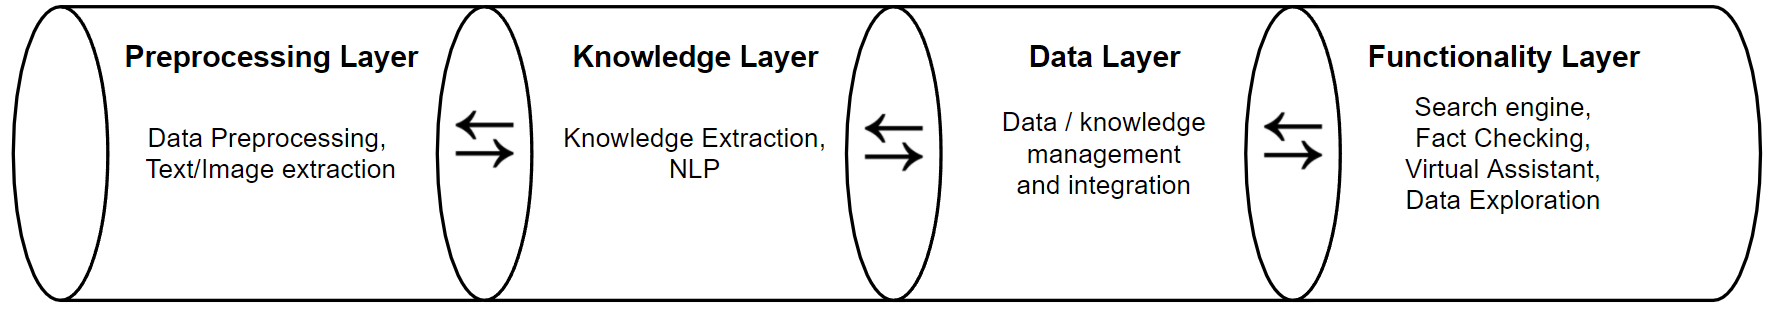
\includegraphics[width=1\textwidth]{Images/Pipeline.PNG}
    \caption{Illustration of the Knox pipeline\label{fig:pipeline}.}
\end{figure}

Last year, a User Interface (UI) layer was introduced. This year, the responsibility of creating UI elements have been split among all groups, who provide interface for their own systems.

\subsubsection{Preprocessing Layer}
The preprocessing layer is responsible for extracting data from \textit{Nordjyske Mediehus} articles and \textit{Grundfos} manuals. Many of these documents are photo scans of old articles, which means that both font, layout, and quality varies from document to document. For this reason, it is necessary to convert many of the documents to a standard format, before it is possible to extract any data. The result should allow all data from \textit{Nordjyske Mediehus} and \textit{Grundfos} to be extracted. 

\subsubsection{Knowledge layer}
The knowledge layer is used to process the data extracted by the preprocessing layer. Methods like Natural Language Processing (NLP) algorithms should be applied to extract knowledge, word count should be tallied and sent to the database, or the text should be annotated to extract entities and their relations, enabling a knowledge graph to be constructed.

\subsubsection{Data layer}\label{databaseResponsibility}
The data layer is responsible for handling the flow of data between the knowledge layer and the functionality layer in the \knox{} pipeline.
New data must be stored on the servers, and it must be accessible to the components that need it. 
This requires close cooperation with the other layers in the pipeline.


As multiple components in the \knox{} system both provide and require access to data, there needs to be a streamlined process for handling this.
In addition, both data storage and access must be handled efficiently.

\subsubsection{Functionality layer}
The purpose of the functionality layer is to use the data from the knowledge layer to apply functionality to the system.
Different kinds of functionalities can be added such as fact-checking, data exploration, search engine, and a virtual assistant.
 The goal for the functionality layer is to provide components, allowing a user to interact with the Knox system. 
